\subsection{Trajectory Analysis}
\label{appx:analyses:trajectory_analysis}

We present additional characterizations of trajectories corresponding to task instances that were successfully resolved by SWE-agent w/ GPT-4 Turbo (unless otherwise specified).

\begin{figure}[ht]
\centering
\begin{minipage}{0.49\textwidth}
    \centering
    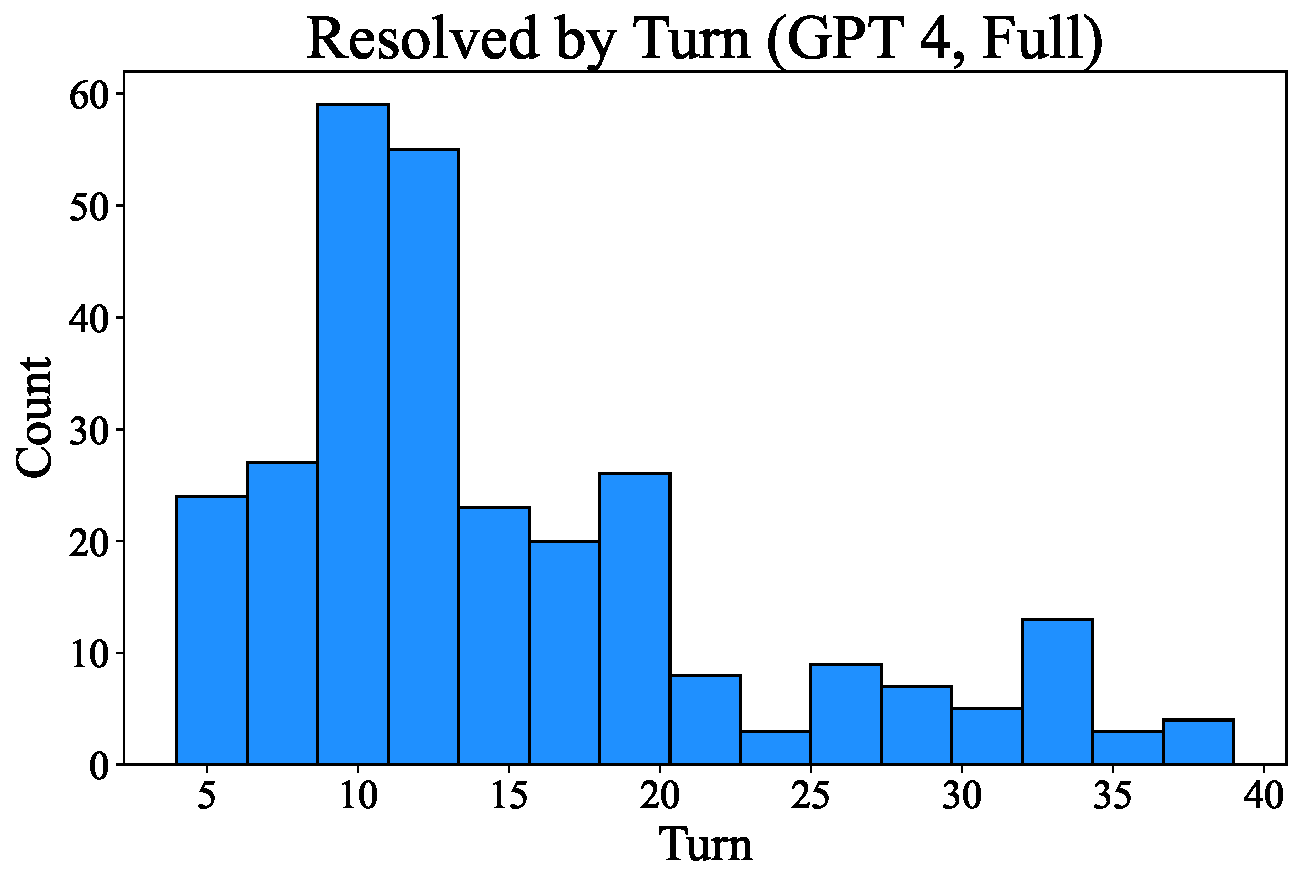
\includegraphics[width=\linewidth]{figures/appx/resolved_by_turn_gpt4.pdf}
\end{minipage}
\begin{minipage}{0.49\textwidth}
    \centering
    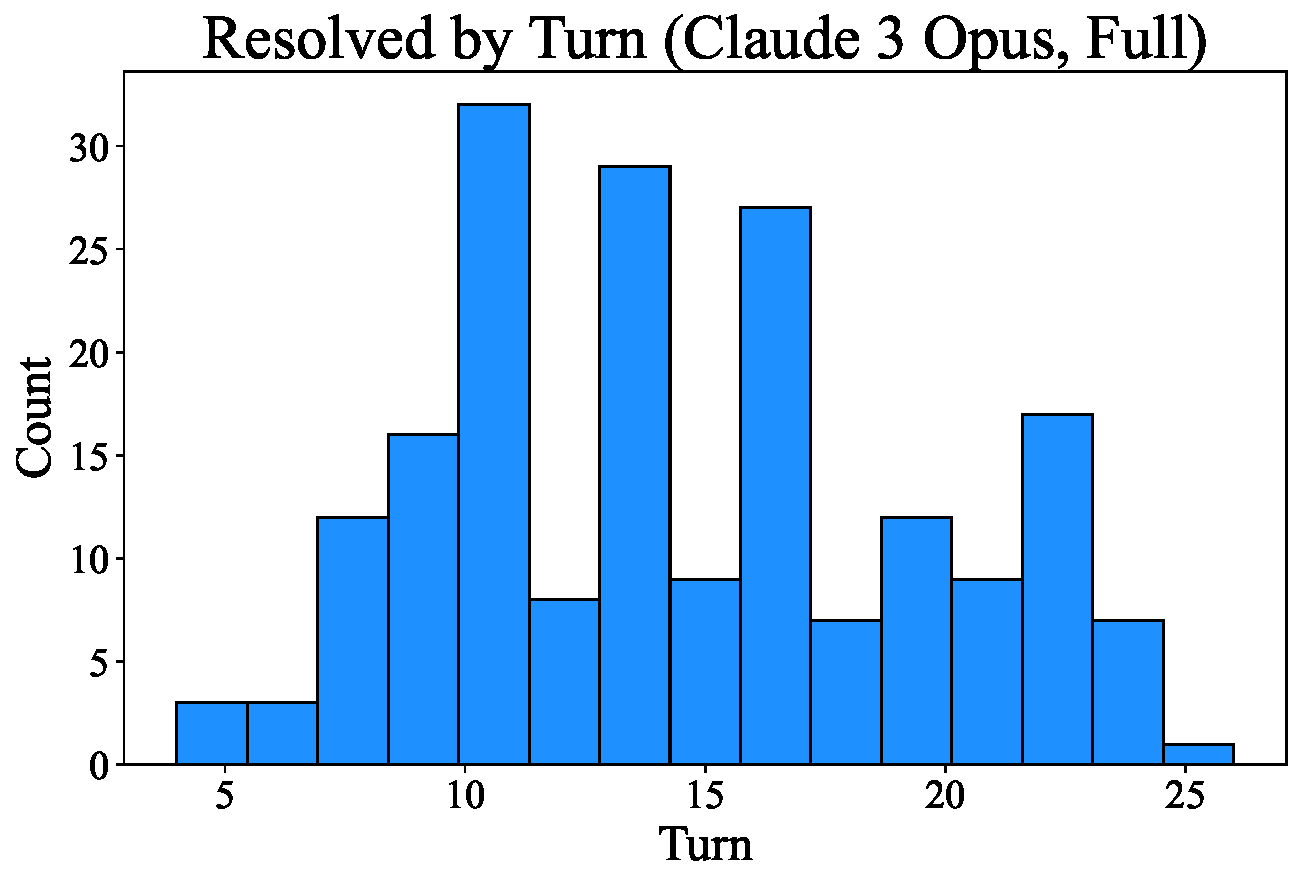
\includegraphics[width=\linewidth]{figures/appx/resolved_by_turn_claude3opus.pdf}
\end{minipage}
\caption{
Distribution of the number of turns for interactive trajectories corresponding to solved task instances on SWE-bench.
The left histogram shows this distribution for SWE-agent w/ GPT 4 on the full SWE-bench test set (286 trajectories).
The right histogram is the performance of SWE-agent w/ Claude 3 Opus on the Lite split of the SWE-bench test set (35 trajectories).
}
\label{fig.resolved_by_turn}
\end{figure}

\begin{figure}[ht]
\centering
\begin{minipage}{0.49\textwidth}
    \centering
    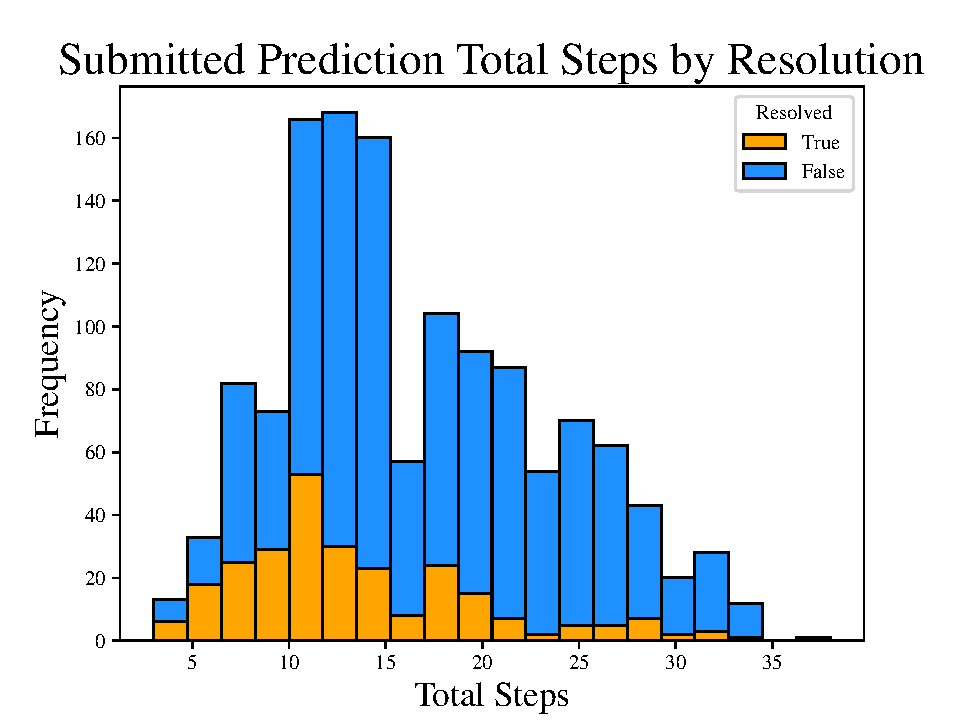
\includegraphics[width=\linewidth]{figures/appx/submitted_steps_x_resolved.pdf}
\end{minipage}
\begin{minipage}{0.49\textwidth}
    \centering
    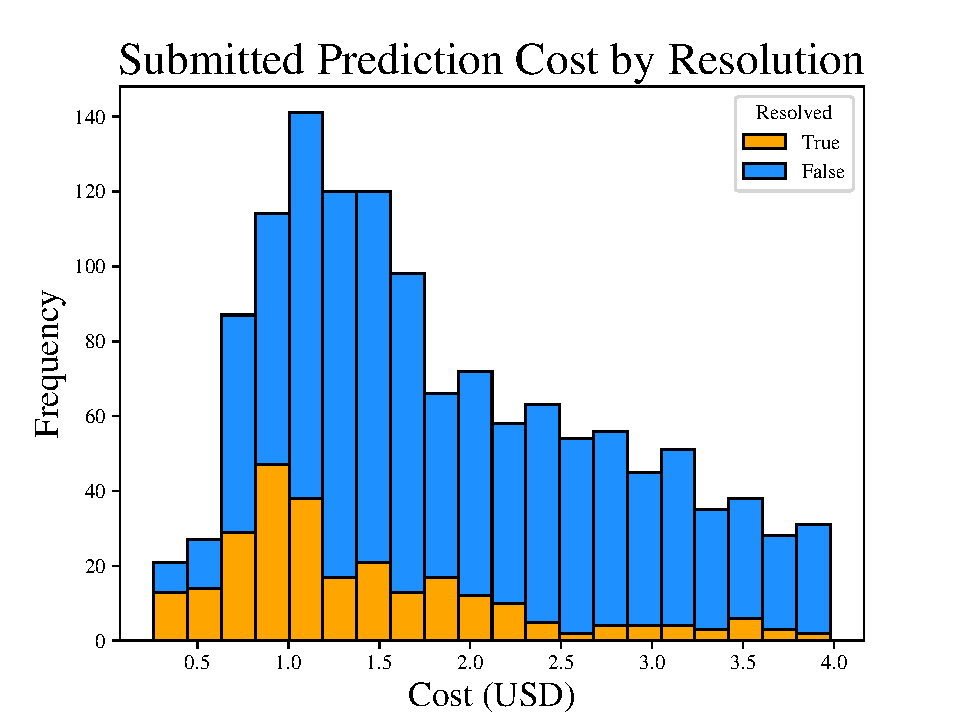
\includegraphics[width=\linewidth]{figures/appx/submitted_cost_x_resolved.pdf}
\end{minipage}
\caption{
The distribution of agent trajectories by total steps (left) and cost (right) for SWE-agent with GPT-4 Turbo on SWE-bench.
The distributions of resolved instances are shown in orange and unresolved are shown in blue.
Resolved instances clearly display an earlier mean and fewer proportion of trajectories with many steps or that cost near the maximum budget of \$$4.00$.
}
\label{fig:appx:steps_vs_cost_resolved}
\end{figure}

\subsubsection{Turns to Resolution}
\label{appx:analyses:trajectory_analysis:turns_to_resolution}
Figure~\ref{fig.resolved_by_turn} visualizes the distribution of the number of turns SWE-agent needed to complete task instances that were successfully resolved.
On the full SWE-bench test set, SWE-agent w/ GPT-4 takes an average of 14.71 turns to finish a trajectory, with a median of 12 turns and 75\% of trajectories being completed within 18 turns.
On the Lite split of the SWE-bench test set, SWE-agent w/ Claude 3 Opus takes an average of 12.71 turns to finish a trajectory, with a median of 13 turns and 75\% of trajectories being completed within 15 turns.
From the distribution, it is evident that across models and SWE-bench splits, the majority of task instances are typically solved and completed comfortably within the allotted budget.

This also points to a general area of improvement for language agent systems --- if a language agent's initial problem solving approach, typically reflected in the first 10 to 20 turns, does not yield a good solution, it struggles to make use of later turns that build upon past mistakes.
To remedy this issue and induce stronger error recovery capabilities in language agents, future directions could consider improving either the model, the ACI, or both.

\begin{table}
    \caption{
We present a table of the most frequently occurring action patterns at each turn (``frequently" means $\geq$ 4 times) in trajectories of task instances resolved by SWE-agent w/ GPT-4.
For instance, the pattern \texttt{create},\texttt{edit},\texttt{python} appears 156 times at the first to third turns.
In addition, we also manually assign each entry a category (Reproduction, Localization (File), Localization (Line), Editing, Submission) that generally captures the underlying purpose of such a pattern.
``Reproduction" refers to the sub-task of recreating the error or request described by the issue.
``Localization" refers to the sub-task of identifying the code that is the cause of the issue.
% ``Editing" refers to the sub-task of editing code such that it fixes the issue.
% ``Submission" refers to the sub-task of checking if an edit resolves the original issue and invoking \texttt{submit} to terminate the episode.
}
    \label{tab:most_common_triples_by_index}
    \vspace{0.25em}
    \centering
    \begin{tabular}{llll}
\toprule
Turns & Pattern & Count & Category \\
\midrule
1-3 & \texttt{create}, \texttt{edit}, \texttt{python} & 156 & Reproduction \\
1-3 & \texttt{search\_dir}, \texttt{open}, \texttt{search\_file} & 21 & Localization (File) \\
1-3 & \texttt{search\_dir}, \texttt{open}, \texttt{scroll\_down} & 12 & Localization (Line) \\
1-3 & \texttt{create}, \texttt{edit}, \texttt{edit} & 11 & Reproduction \\
1-3 & \texttt{search\_dir}, \texttt{open}, \texttt{edit} & 10 & Localization (Line) \\
2-4 & \texttt{edit}, \texttt{python}, \texttt{find\_file} & 71 & Localization (File) \\
2-4 & \texttt{edit}, \texttt{python}, \texttt{edit} & 37 & Reproduction \\
2-4 & \texttt{edit}, \texttt{python}, \texttt{search\_dir} & 26 & Localization (File) \\
2-4 & \texttt{edit}, \texttt{python}, \texttt{open} & 15 & Localization (File) \\
2-4 & \texttt{open}, \texttt{edit}, \texttt{edit} & 13 & Editing \\
2-4 & \texttt{open}, \texttt{edit}, \texttt{create} & 13 & Editing \\
2-4 & \texttt{open}, \texttt{scroll\_down}, \texttt{scroll\_down} & 9 & Localization (Line) \\
2-4 & \texttt{open}, \texttt{scroll\_down}, \texttt{edit} & 5 & Editing \\
2-4 & \texttt{open}, \texttt{edit}, \texttt{submit} & 5 & Submission \\
3-5 & \texttt{python}, \texttt{find\_file}, \texttt{open} & 61 & Localization (File) \\
3-5 & \texttt{python}, \texttt{edit}, \texttt{python} & 25 & Editing \\
3-5 & \texttt{search\_file}, \texttt{goto}, \texttt{edit} & 24 & Localization (Line) \\
3-5 & \texttt{python}, \texttt{search\_dir}, \texttt{open} & 23 & Localization (File) \\
3-5 & \texttt{edit}, \texttt{create}, \texttt{edit} & 13 & Editing \\
3-5 & \texttt{python}, \texttt{edit}, \texttt{edit} & 11 & Editing \\
3-5 & \texttt{python}, \texttt{open}, \texttt{edit} & 7 & Editing \\
3-5 & \texttt{python}, \texttt{find\_file}, \texttt{find\_file} & 7 & Localization (File) \\
3-5 & \texttt{edit}, \texttt{edit}, \texttt{submit} & 4 & Submission \\
3-5 & \texttt{edit}, \texttt{edit}, \texttt{create} & 4 & Editing \\
4-6 & \texttt{find\_file}, \texttt{open}, \texttt{edit} & 28 & Editing \\
4-6 & \texttt{find\_file}, \texttt{open}, \texttt{search\_file} & 19 & Localization (Line) \\
4-6 & \texttt{edit}, \texttt{edit}, \texttt{python} & 11 & Reproduction \\
4-6 & \texttt{goto}, \texttt{edit}, \texttt{edit} & 8 & Editing \\
4-6 & \texttt{find\_file}, \texttt{open}, \texttt{goto} & 8 & Localization (Line) \\
4-6 & \texttt{goto}, \texttt{edit}, \texttt{submit} & 7 & Submission \\
4-6 & \texttt{goto}, \texttt{edit}, \texttt{create} & 7 & Editing \\
4-6 & \texttt{find\_file}, \texttt{open}, \texttt{scroll\_down} & 6 & Localization (Line) \\
4-6 & \texttt{scroll\_down}, \texttt{scroll\_down}, \texttt{edit} & 5 & Localization (Line) \\
4-6 & \texttt{find\_file}, \texttt{find\_file}, \texttt{open} & 5 & Localization (File) \\
5-7 & \texttt{open}, \texttt{search\_file}, \texttt{goto} & 29 & Localization (Line) \\
5-7 & \texttt{open}, \texttt{edit}, \texttt{python} & 20 & Editing \\
5-7 & \texttt{open}, \texttt{goto}, \texttt{edit} & 7 & Editing \\
5-7 & \texttt{scroll\_down}, \texttt{edit}, \texttt{submit} & 4 & Submission \\
6-8 & \texttt{scroll\_down} (x3) & 6 & Localization (Line) \\
6-8 & \texttt{search\_file}, \texttt{goto}, \texttt{scroll\_down} & 4 & Localization (Line) \\
7-9 & \texttt{edit}, \texttt{python}, \texttt{rm} & 20 & Editing \\
7-9 & \texttt{goto}, \texttt{edit}, \texttt{python} & 12 & Editing \\
8-10 & \texttt{python}, \texttt{rm}, \texttt{submit} & 19 & Submission \\
8-10 & \texttt{search\_file}, \texttt{goto}, \texttt{search\_file} & 4 & Localization (File) \\
9-11 & \texttt{edit} (x3) & 18 & Editing \\
9-11 & \texttt{edit}, \texttt{open}, \texttt{edit} & 6 & Editing \\
9-11 & \texttt{goto}, \texttt{search\_file}, \texttt{goto} & 4 & Localization (Line) \\
\bottomrule
    \end{tabular}
\end{table}

\subsubsection{Walkthrough of Trajectory Phases}
\label{appx:analyses:trajectory_analysis:walkthrough}
We describe what happens in different phases of an agent's problem solving trajectory.
To support our observations, we present several tables and distributions that help highlight consistent trends.

\begin{figure}
    \centering
    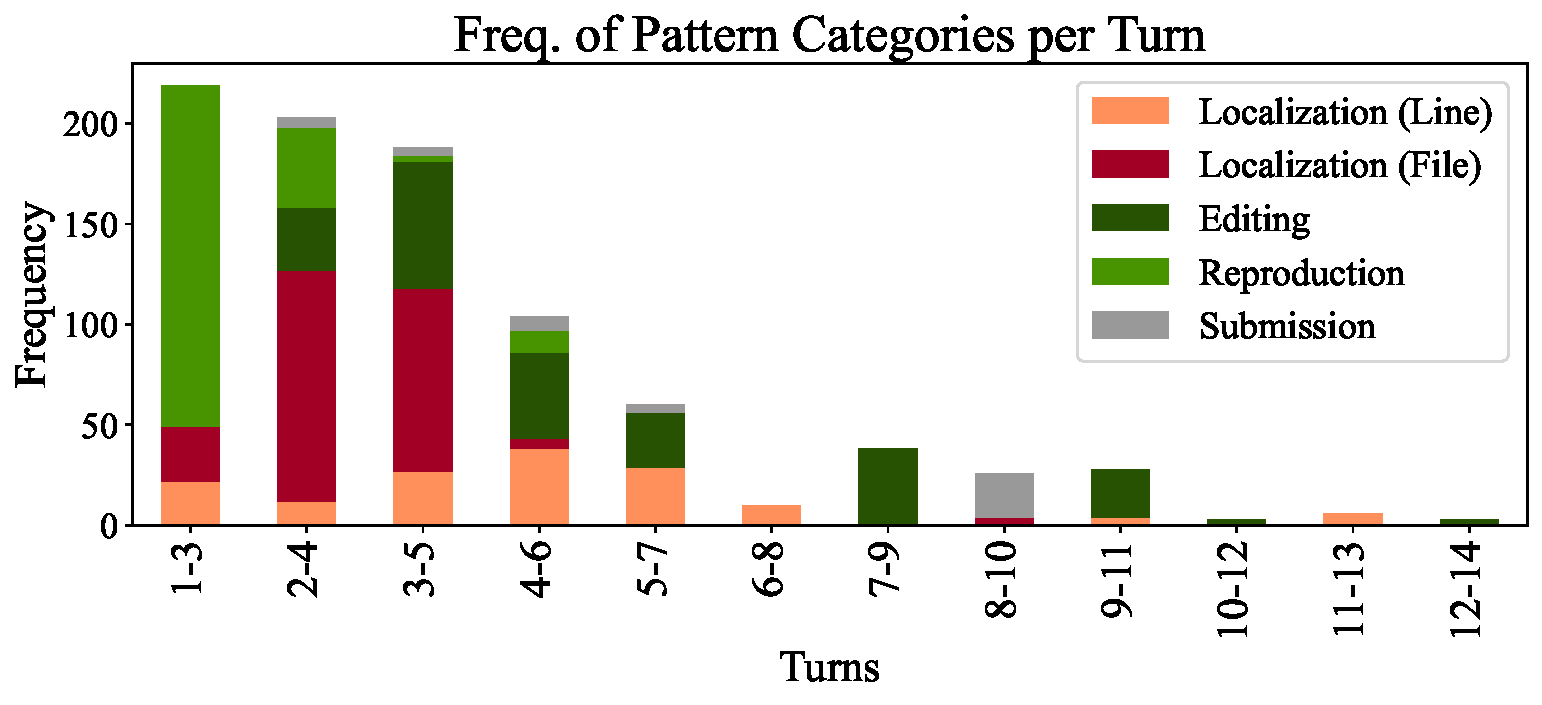
\includegraphics[width=\textwidth]{figures/appx/categories_per_turns.pdf}
    \caption{We assign each pattern to one of five categories (as presented in Table~\ref{tab:most_common_triples_by_index}) and present a histogram of the turns at which patterns from specific categories show up frequently.}
    \label{fig.pattern_categories_per_turns}
\end{figure}


\textbf{Initial reproduction, localization steps.} First, the initial steps that SWE-agent usually takes is heavily dominated by Localization and Reproduction operations.
The most commonly occurring pattern in general is the \texttt{create}, \texttt{edit}, \texttt{python} triplet.
Across these commands, an agent creates an empty python file, adds an executable code snippet via \texttt{edit}, and then attempts to run it.
As an alternative, the agent also sometimes decides to start off instead with Localization, or identifying the files/lines causing the issue.
Depending on how informative the issue description and results for initial search queries are, agents will run additional search queries with finer grained search tools to zoom in on the target problematic code area (e.g., \texttt{search\_dir}, \texttt{open}, \texttt{search\_file}/\texttt{scroll\_down}).

These trends are also reflected in Figure~\ref{fig.pattern_categories_per_turns}, which shows a distribution of patterns across turns according to the categories defined in Table~\ref{tab:most_common_triples_by_index}.
The three leftmost bars reflect that Reproduction followed by Localization constitutes the lion's share of operations that occur in the early phases of a trajectory.
For a more thorough breakdown, we also include Figure~\ref{fig.actions_per_turn_density}, which shows an estimated distribution of each action with respect to different turns, normalized across the total number of times the command occurs across all turns.
From these graphs, we can see that \texttt{create} is invoked much more frequently in the very first turn than in any other turn.
The \texttt{search\_dir} and \texttt{search\_file} distributions are roughly bi-modal, with a peak of occurrences for both actions showing up in Turn 1 (if the agent decides to do Localization immediately) and the Turn 4 (if the agent decides to do Localization after Reproduction).
We also present Figure~\ref{fig.actions_per_turn_norm}, which communicates similar information as Figure~\ref{fig.actions_per_turn_density}, but presented instead as a stacked bar chart with more commands.
The chart is created directly from Figure~\ref{fig:actions_per_turn}, with the frequency of actions at each turn \texttt{n} normalized across the total number of trajectories with a length greater than or equal to \texttt{n} turns.

\begin{figure}[ht]
    \centering
    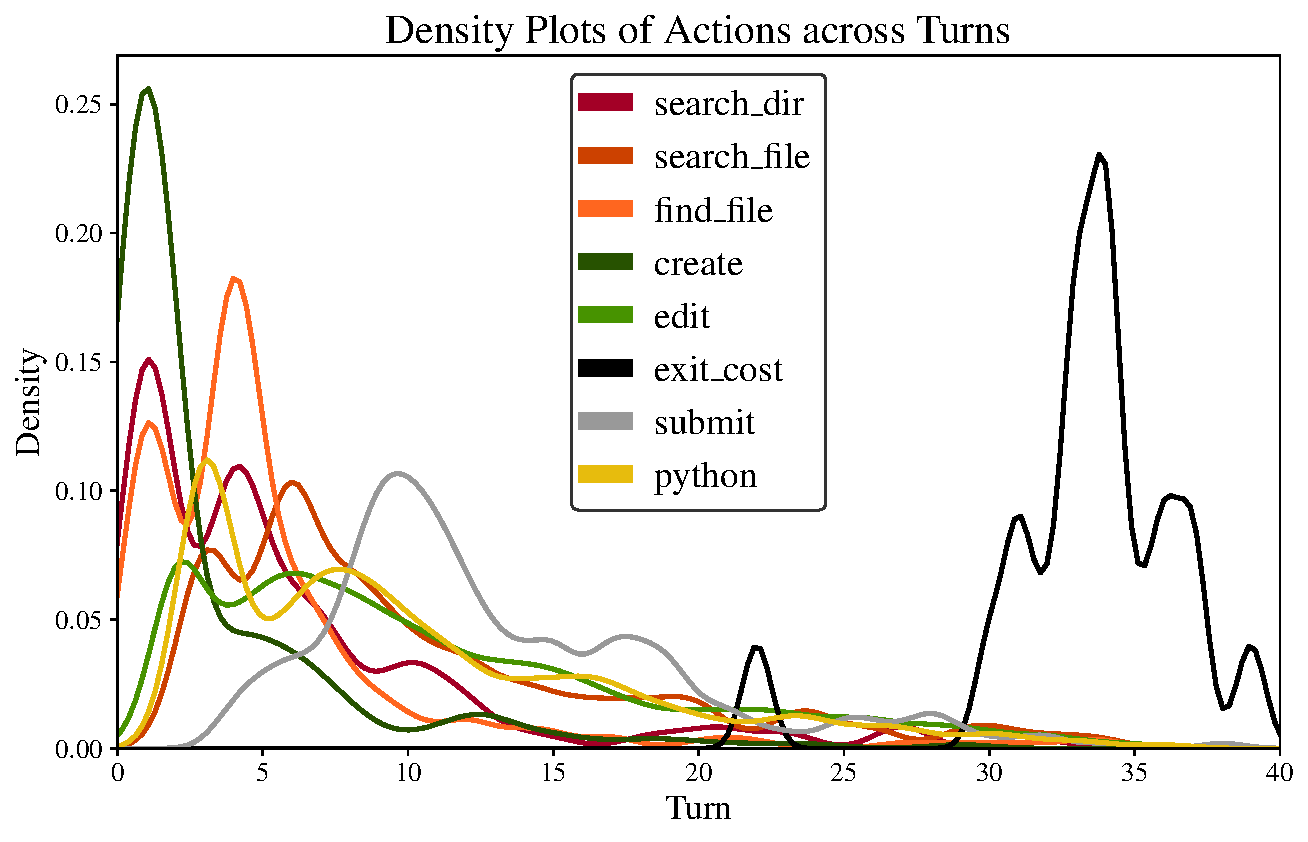
\includegraphics[width=0.9\linewidth]{figures/appx/actions_per_turn_dist.pdf}
    \caption{This density plot shows a normalized distribution of actions across different turns of a trajectory. \texttt{exit\_cost} refers to when the token budget cost was exhausted and the episode's changes are automatically submitted (contrary to an intentional \texttt{submit} invoked by the agent).}
    \label{fig.actions_per_turn_density}
\end{figure}

\textbf{Cycle of edit, then evaluate.} From the fifth turn onwards, the distribution of actions per turn can be generally described as alternating \texttt{edit} and \texttt{python}/\texttt{pytest} actions.
After reproducing the issue and localizing the file(s) responsible for the problem, agents will typically make edits to the file, then run the reproduction script or existing tests to check whether the proposed edits resolve the original issue and maintain existing desirable behavior.
This pair of actions will often repeat for several turns, as an initial edit usually does not successfully resolve the given issue.
Multiple rounds of editing that are supplemented by execution feedback from prior turns are conducive to more well-formed, successful subsequent edits.
As reflected in Table~\ref{tab:most_common_triples_by_index}, for turn 4 onwards, the most popular pattern that begins at each turn usually falls under the Editing category.
This is also made obvious by Figure~\ref{fig.actions_per_turn_norm}, where the \texttt{edit} command is the most popular command for Turns \num{5} to \num{31}, with only one exception (Turn \num{30}).
From Figure~\ref{fig.actions_per_turn_density}, it is also notably that the distributions of the \texttt{edit} and \texttt{python} commands are quite similar, as they typically follow one another.

\begin{figure}[ht]
    \centering
    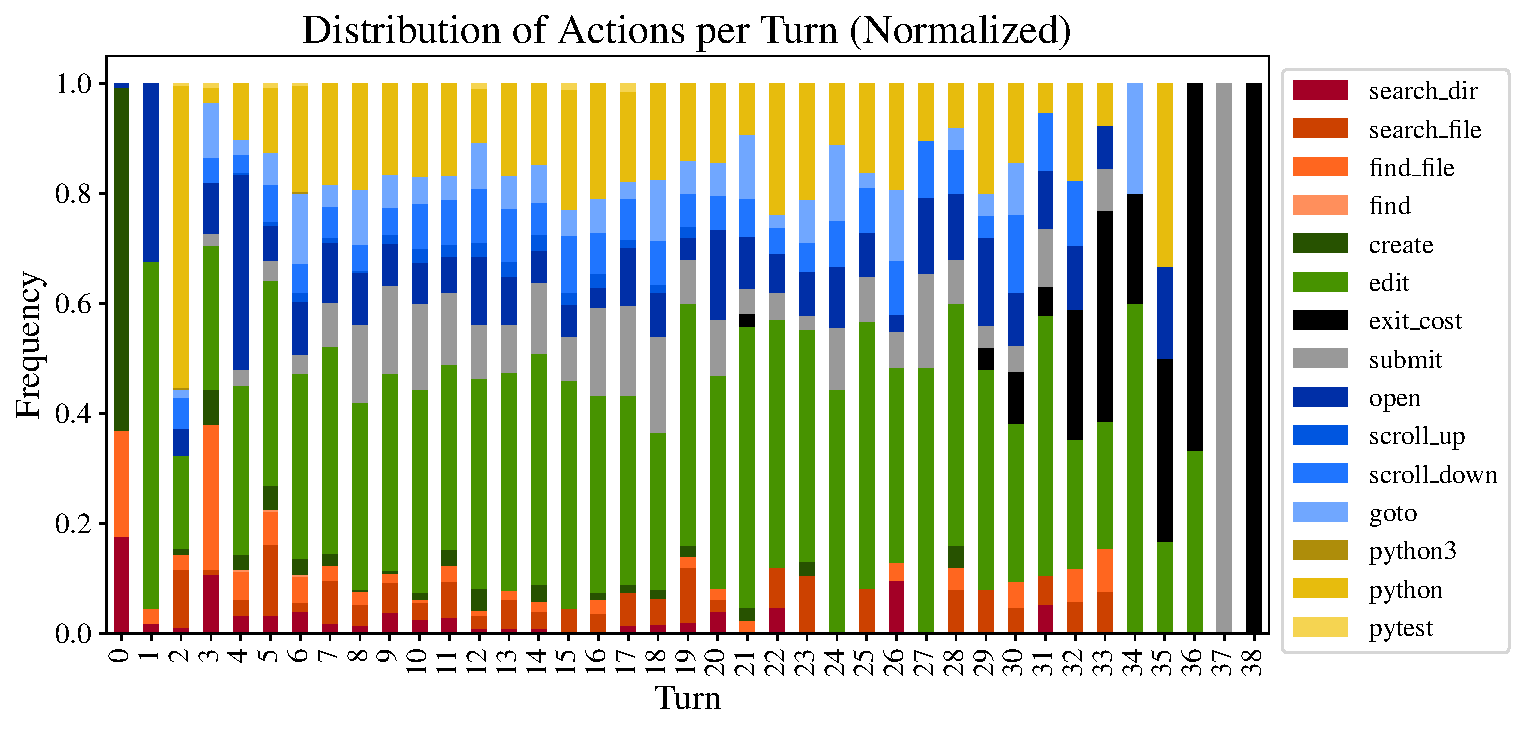
\includegraphics[width=\linewidth]{figures/appx/actions_per_turn_norm.pdf}
    \caption{
    A normalized view of Figure~\ref{fig:actions_per_turn}. 
    The distributions for turn \texttt{n} are normalized across the number of trajectories that have a length of at least \texttt{n} or more turns.
    }
    \label{fig.actions_per_turn_norm}
\end{figure}

Interspersed across these later turns are additional Localization operations for inspecting other parts of the current file (e.g., \texttt{scroll\_down}, \texttt{scroll\_up}) or opening other files (e.g., \texttt{open}, \texttt{search\_dir/file}, \texttt{find\_file}).
These minor trend lines reflect the tasks that involve multi-line or multi-file edits.
Figure~\ref{fig.actions_per_turn_norm} displays a steady presence of such actions from Turn \num{6} onwards.
Agents will invoke such actions to read different parts (e.g., documentation, implementation) of a long function, especially when it does not fit entirely within the file viewer's number of lines.
After editing one function \texttt{A}, running the reproduction script will occasionally propagate an error in a different function \texttt{B}, where function \texttt{B} invokes \texttt{A}.
This is a common reason for the additional directory and file level navigation that occurs in the later stages of a trajectory.

\textbf{Concluding submission turns.} 
There is a consistent proportion of \texttt{submit} actions per turn, with a relative peak around Turn \num{10}, as shown in Figure~\ref{fig.actions_per_turn_density}.
As mentioned in Section~\ref{sec:analysis:agent-behavior} and above, the majority of resolved task instances end with an intentional \texttt{submit} command.
As suggested by both Figure~\ref{fig:appx:steps_vs_cost_resolved} and Figure~\ref{fig.actions_per_turn_norm}, submissions are concentrated between Turns \num{10} and \num{20}, becoming less frequent for each turn beyond this range.
This trend reflects how agents struggle to use later turns to their advantage, particularly when the original problem solving approach fails, which is fairly evident by Turn~\num{20}.
Effectively utilizing later turns to either remedy multiple prior errors or pivot to a different problem solving approach are all viable strategies given the \num{20}+ turns that remain.
However, due to overwhelming context or greedy tendencies, agents do not reflect such dynamic behavior, instead opting to focus on continued local editing rather than additional exploration.

Finally, there is a sharp cut off of \texttt{exit\_cost} actions scattered throughout Turns \num{30} to \num{40}; this reflects that the \$\num{4} cost limit we impose on runs roughly corresponds to this number of turns.
The discrepancies mainly comes from variations in the size of observations, with trajectories containing multiple observations that have a high number of tokens corresponding to ones that terminate relatively earlier.
Increasing the cost allowance per task episode would directly increase the maximum number of the turns per episode.

\subsubsection{Breakdowns of Action Sequences}
\label{appx:analyses:trajectory_analysis:action_breakdown}
In this part, we include more granular examinations of patterns of actions that emerge frequently in trajectories.
We also identify consistent associations between groups of actions and how their effects build off one another across several turns.

\textbf{Editing Trends.}
Editing is a core facet of agents' ability to reproduce issues and propose fixes effectively. 
It is also the action that models typically struggle with the most.
Here, we list several trends we were able to discern about how agents edit.

First, across the full SWE-bench test set, a non-trivial minority of edit actions are unsuccessful, meaning the \texttt{edit} invocation raises a linting error.
Going forwards, we refer to such an occurrence as a \textit{failed} edit.
Out of \num{2294} task instances, \num{1185} (\num{51.7}\%) have at least one turn with an failed edit.
Of these trajectories, there is a median of \num{3} failed edits per trajectory, with a max of \num{33}.
The rate of failed edits is smaller for resolved task instances.
Out of \num{286} resolved instances, \num{113} (\num{31.5}\%) have at least one turn with an failed edit, with a median/mean/max of \num{2} failed edits per trajectory, with a max of \num{26}.
Figure~\ref{fig.failed_edits_per_traj} shows corresponding distributions.

\begin{figure}[ht]
    \centering
    \begin{subfigure}[b]{0.49\textwidth}
        \centering
        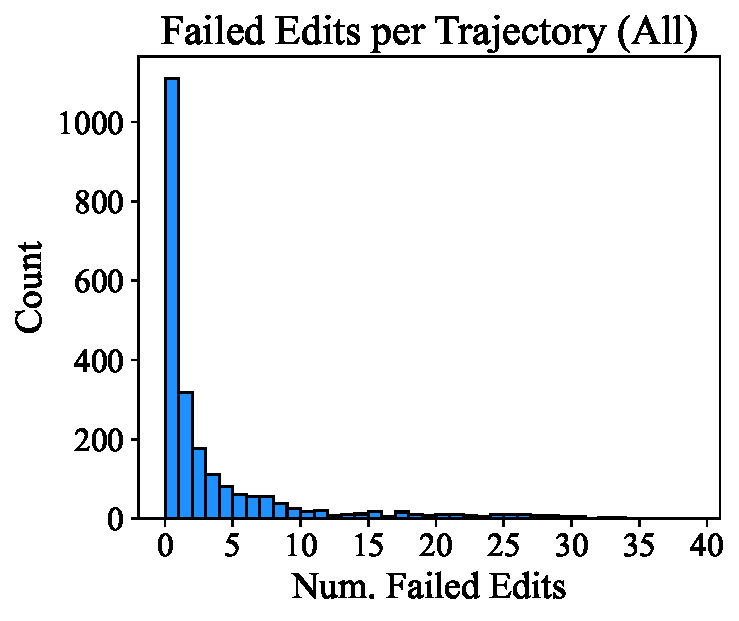
\includegraphics[width=\textwidth]{figures/appx/failed_edits_per_trajectory.pdf}
    \end{subfigure}
    \begin{subfigure}[b]{0.49\textwidth}
        \centering
        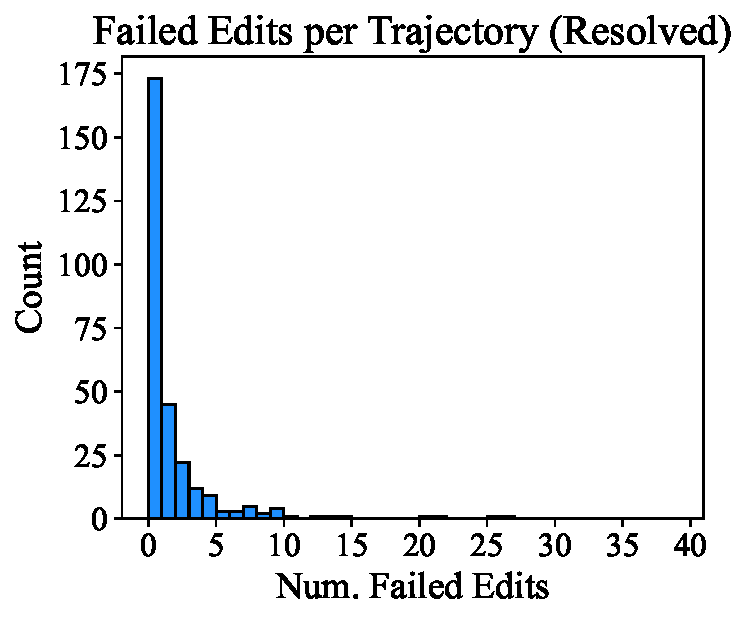
\includegraphics[width=\textwidth]{figures/appx/failed_edits_per_trajectory_resolved.pdf}
    \end{subfigure}
    \caption{
    Distribution of the number of failed \texttt{edit} actions per trajectory across all (left) and resolved (right) task instances by SWE-agent with GPT-4 Turbo.
    A ``failed" edit refers to an edit action that raised a linting error.
    The left-most bar for both graphs corresponds to the number of trajectories with no failed edits.
    }
    \label{fig.failed_edits_per_traj}
\end{figure}

Second, with linting enabled editing, agents ``recover" more often than not from failed edits.
To understand whether and how effectively agents use linting error feedback to construct a subsequent, well-formed \texttt{edit} action, we define two terms.
Recovery refers to a sequence of failed edits followed immediately by a successful edit, suggesting the agent used linting feedback to make a well-formatted edit.
An unsuccessful recovery is consecutive failed edits followed immediately by a non-edit action.

\begin{figure}[ht]
    \centering
    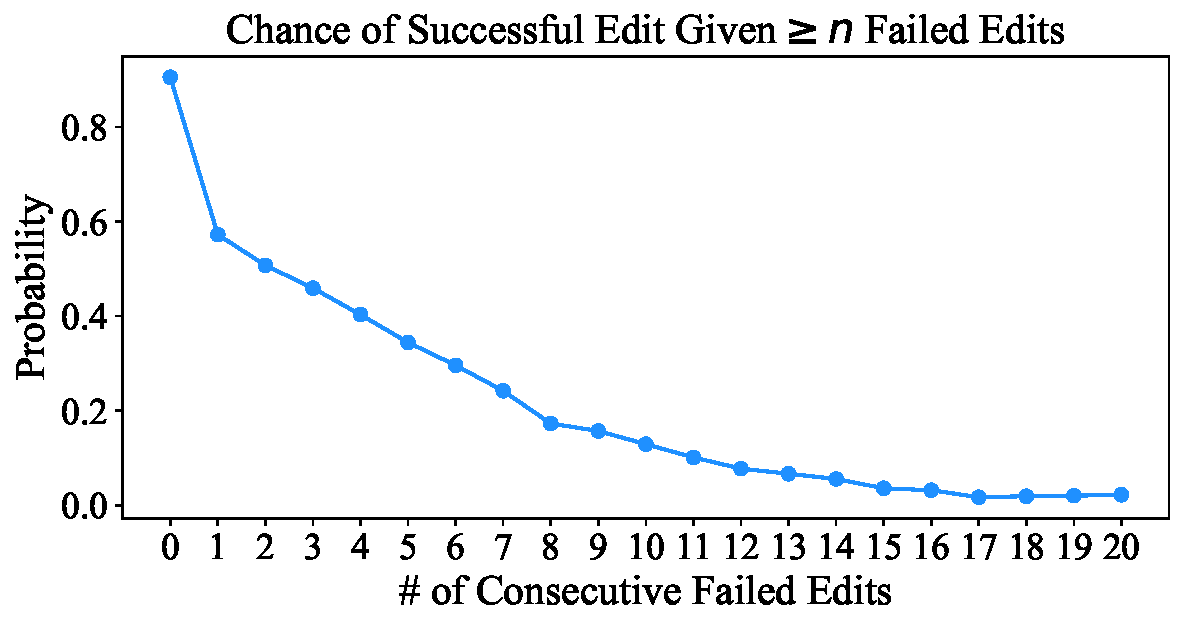
\includegraphics[width=0.6\linewidth]{figures/appx/prob_good_edit_given_n_fails.pdf}
    \caption{
    Probability of successful edit after \texttt{n} failed edits.
    The likelihood of recovery decreases as \texttt{n} increases.
    }
    \label{fig.prob_good_edit_given_n_fails}
\end{figure}

Across trajectories corresponding to resolved task instances, there are \num{135} occurrences of \num{1}+ failed edit attempts.
Out of these, the agent recovers successfully \num{104} times.
The number of consecutive failed edit attempts before a successful versus failed recovery is also vastly different.
Successful recoveries are usually preceded by \num{2.03} edit attempts, less than the average \num{4.22} failed edit attempts of unsuccessful recoveries.
Across all task instances, the relative rate of unsuccessful recoveries increases, with \num{810} successful recoveries versus \num{555} unsuccessful ones.
While the number of consecutive failed edit attempts resulting in a recovery remains steady (\num{2.2}), it increases significantly for unsuccessful recoveries (\num{5.59}).

Third, the odds of recovery decreases as the agent accumulates more failed edit attempts.
Figure~\ref{fig.prob_good_edit_given_n_fails} displays a line plot of the probability of a successful edit given \texttt{n} failed edit attempts in a row.
The leftmost data point of \texttt{n} $=$ \num{0} means that any attempt at editing has a \num{90.5}\% chance of eventually being successful.
This value drops off once the agent incurs a single failed edit; there is only a \num{57.2}\% chance the edit is ultimately successful.
In other words, there is a \num{42.8}\% chance the agent never recovers upon encountering \num{1} edit error.

\textbf{Action sequence analysis.}
We calculate the transition probabilities showing the likelihood of the next action given the previous \texttt{n} actions.
To perform this analysis, we first determine the \num{15} most commonly occurring sequences of \texttt{n} actions, for \texttt{n} $\in\{1, 2, 3, 4\}$.
We then count how frequently each command appears after this sequence and finally normalize the counts across the total number of occurrences of the sequence to get a likelihood of the ``Next Action" with respect to the preceding \texttt{n} sequence of actions.

We show these transition probability heatmaps, with \texttt{n} $=1$ in Figure~\ref{fig:transition_probs}, \texttt{n} $=2$ in Figure~\ref{fig:transition_probs_2gram}, \texttt{n} $=3$ in Figure~\ref{fig:transition_probs_3gram}, and \texttt{n} $=4$ in Figure~\ref{fig:transition_probs_4gram}.
From these graphs, it is immediately obvious that several action sequences emerge consistently across many task instances.
The high likelihood cells in these heatmaps suggest that SWE-agent uses common problem solving patterns which correspond to higher order operations such as reproducing an issue, localizing buggy code, and proposing/verifying edits.

In Figure~\ref{fig:transition_probs}, we see direct associations between pairs of actions.
There are several obvious trends.
All trajectories begin with \texttt{create}, \texttt{find\_file}, \texttt{search\_dir}, and end on either a \texttt{submit} or \texttt{exit\_cost}.
The most popular next action is \texttt{edit}; it is the most likely action to follow \texttt{create}, \texttt{edit}, \texttt{goto}, \texttt{pytest}, and \texttt{python}.
Scroll (e.g., \texttt{scroll\_down/up}) and search (e.g. \texttt{find\_file}, \texttt{search\_dir}) actions tend to be repeated.

\begin{figure}[htbp]
    \centering
    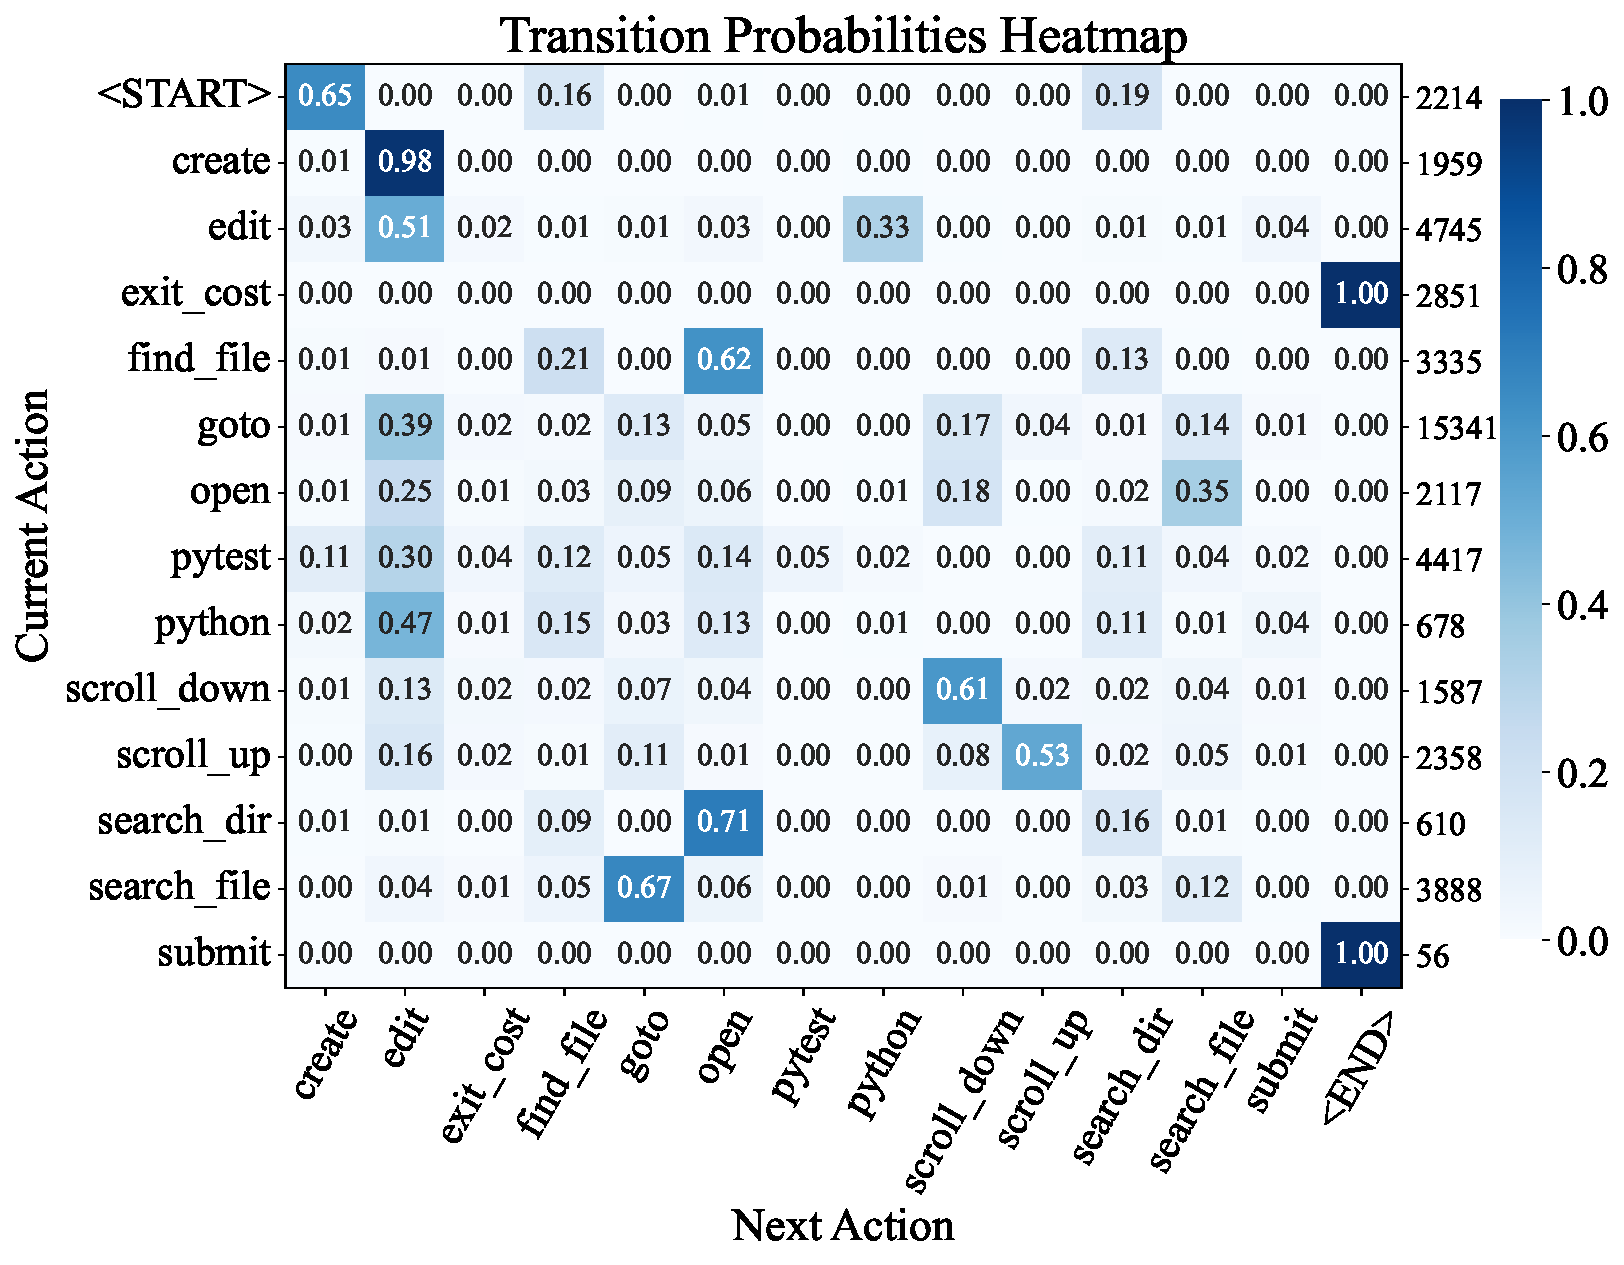
\includegraphics[width=0.9\textwidth]{figures/appx/transition_probs.pdf}
    \caption{
    Heatmap displaying the relative frequency of different actions being invoked after the most popular actions in SWE-agent w/ GPT-4 Turbo trajectories across all task instances.
    }
    \label{fig:transition_probs}
    \vspace{0.5em}
    \centering
    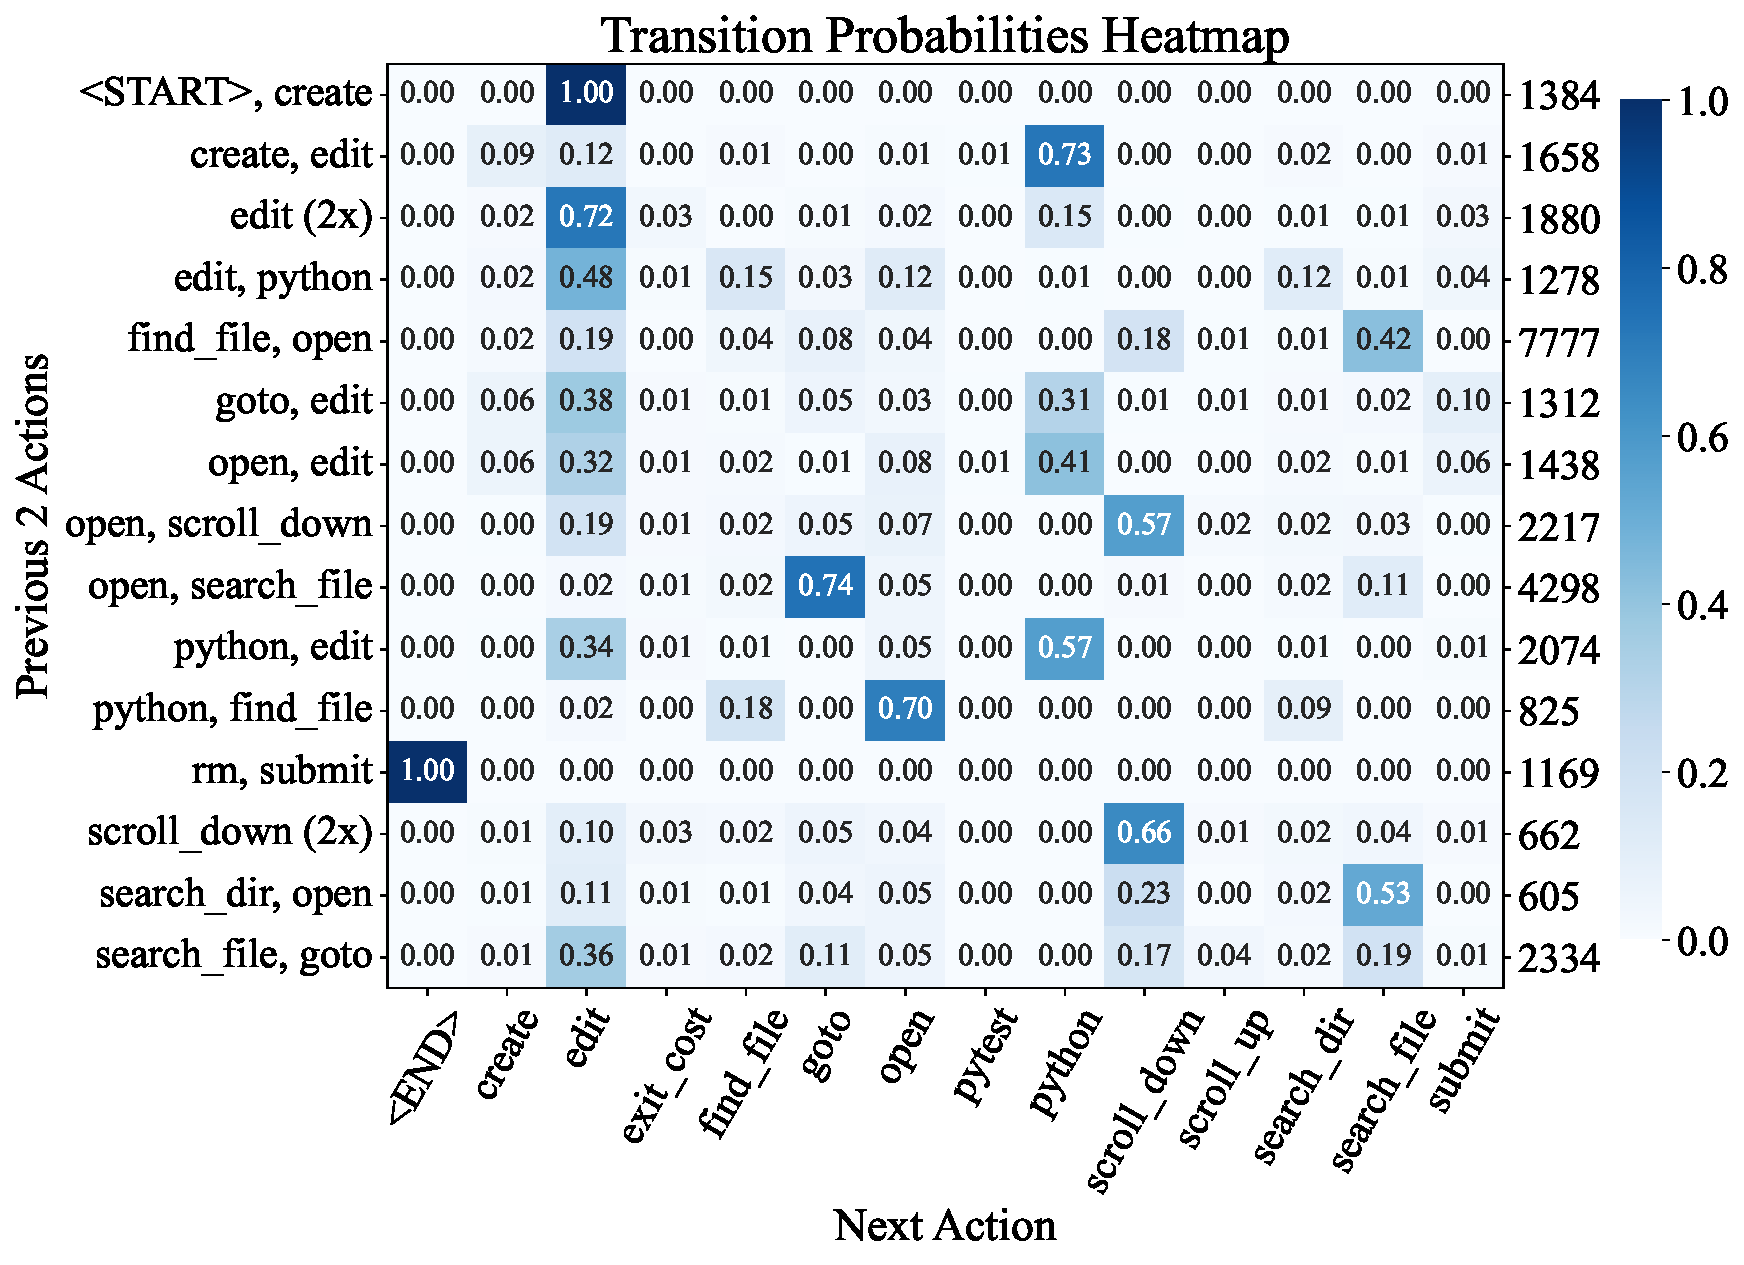
\includegraphics[width=0.9\textwidth]{figures/appx/transition_probs_2gram.pdf}
    \caption{
    Heatmap displaying the relative frequency of different actions being invoked after the most popular \textit{pairs} of actions in SWE-agent w/ GPT-4 Turbo trajectories across all task instances.
    }
    \label{fig:transition_probs_2gram}
\end{figure}
\begin{figure}[htbp]
    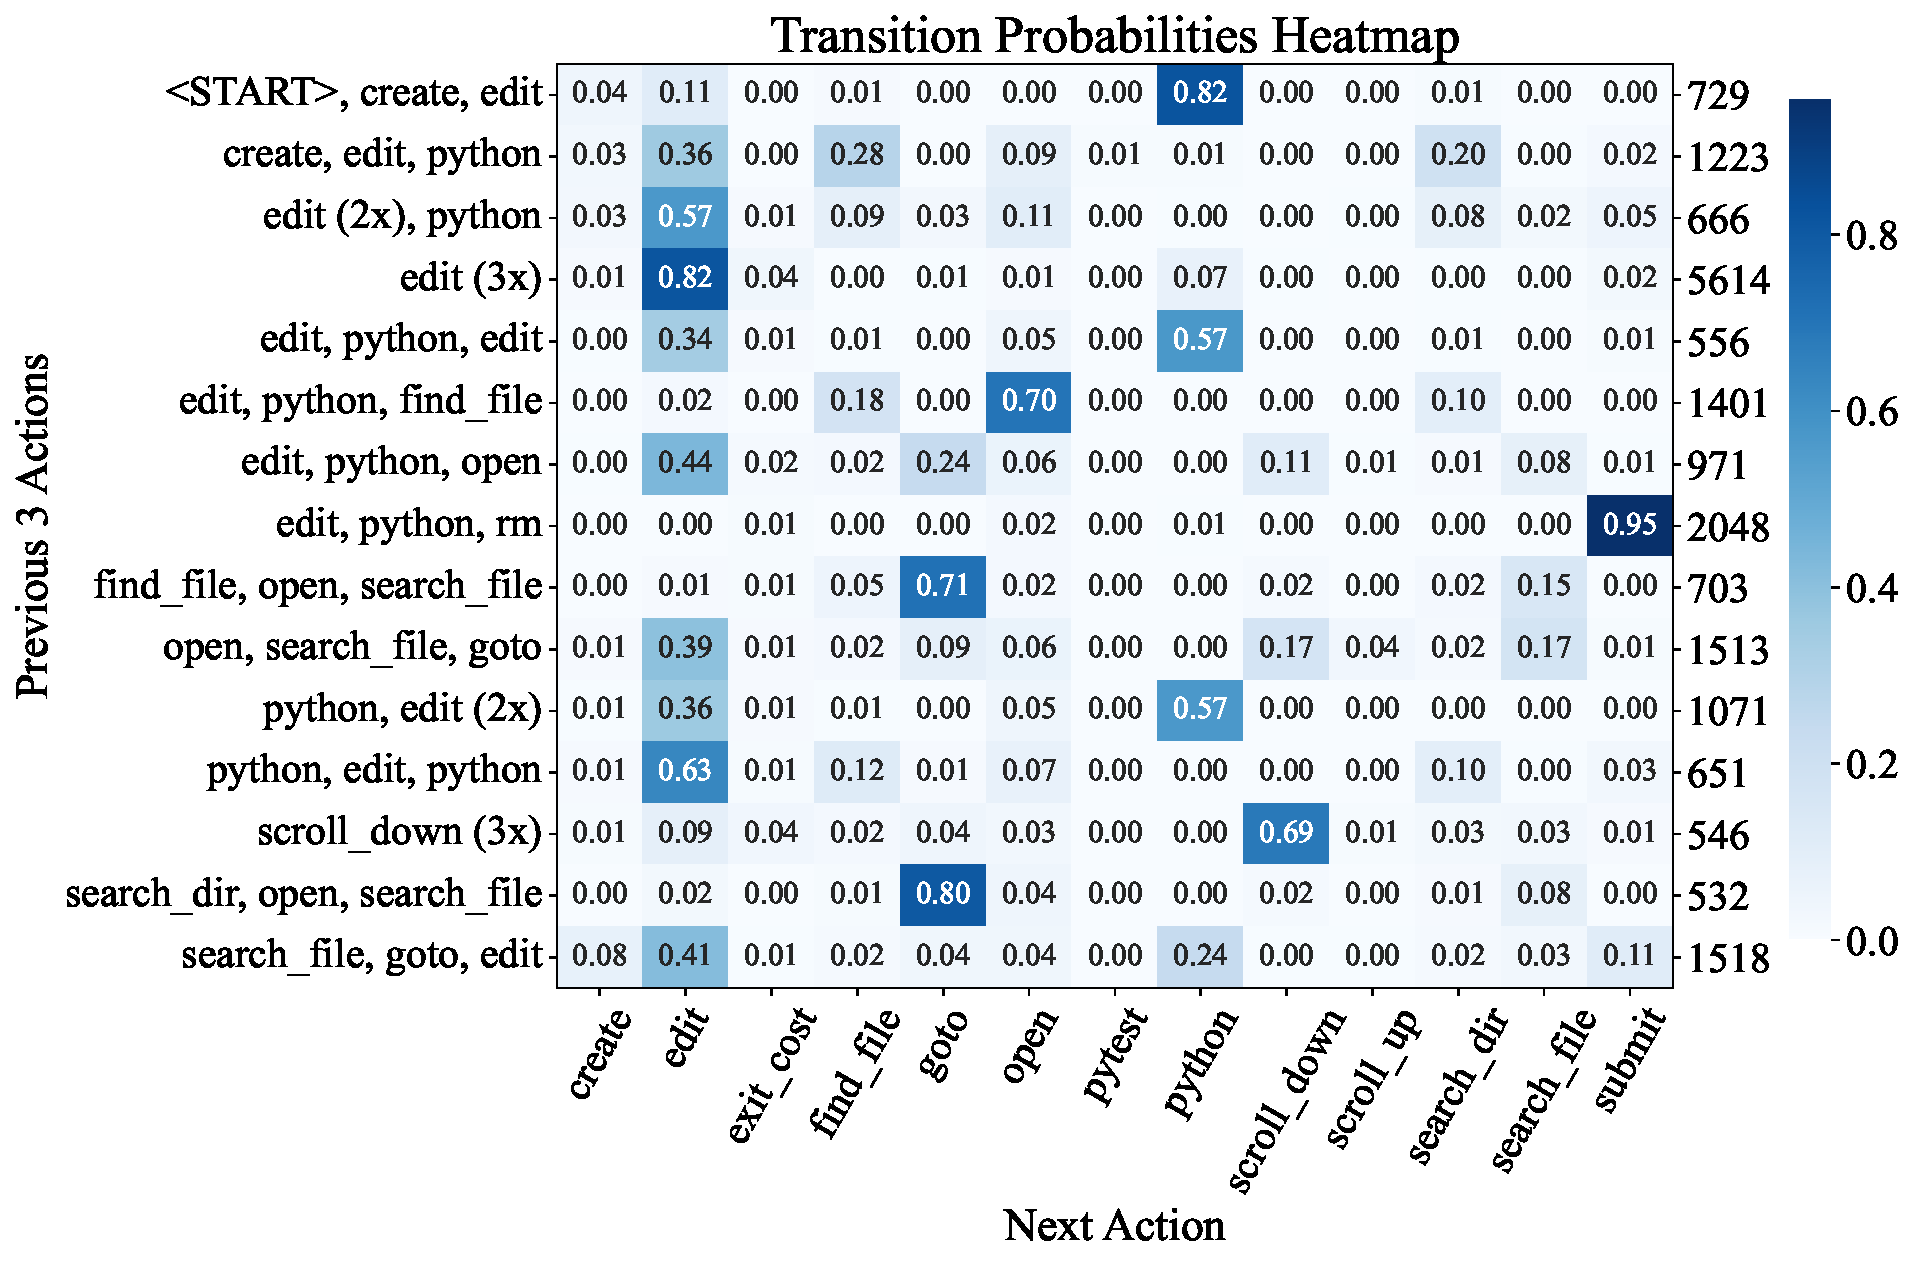
\includegraphics[width=\textwidth]{figures/appx/transition_probs_3gram.pdf}
    \caption{
    Heatmap displaying the relative frequency of different actions being invoked after the most popular \textit{triplets} of actions in SWE-agent w/ GPT-4 Turbo trajectories across all task instances.
    }
    \label{fig:transition_probs_3gram}
    \vspace{1em}
    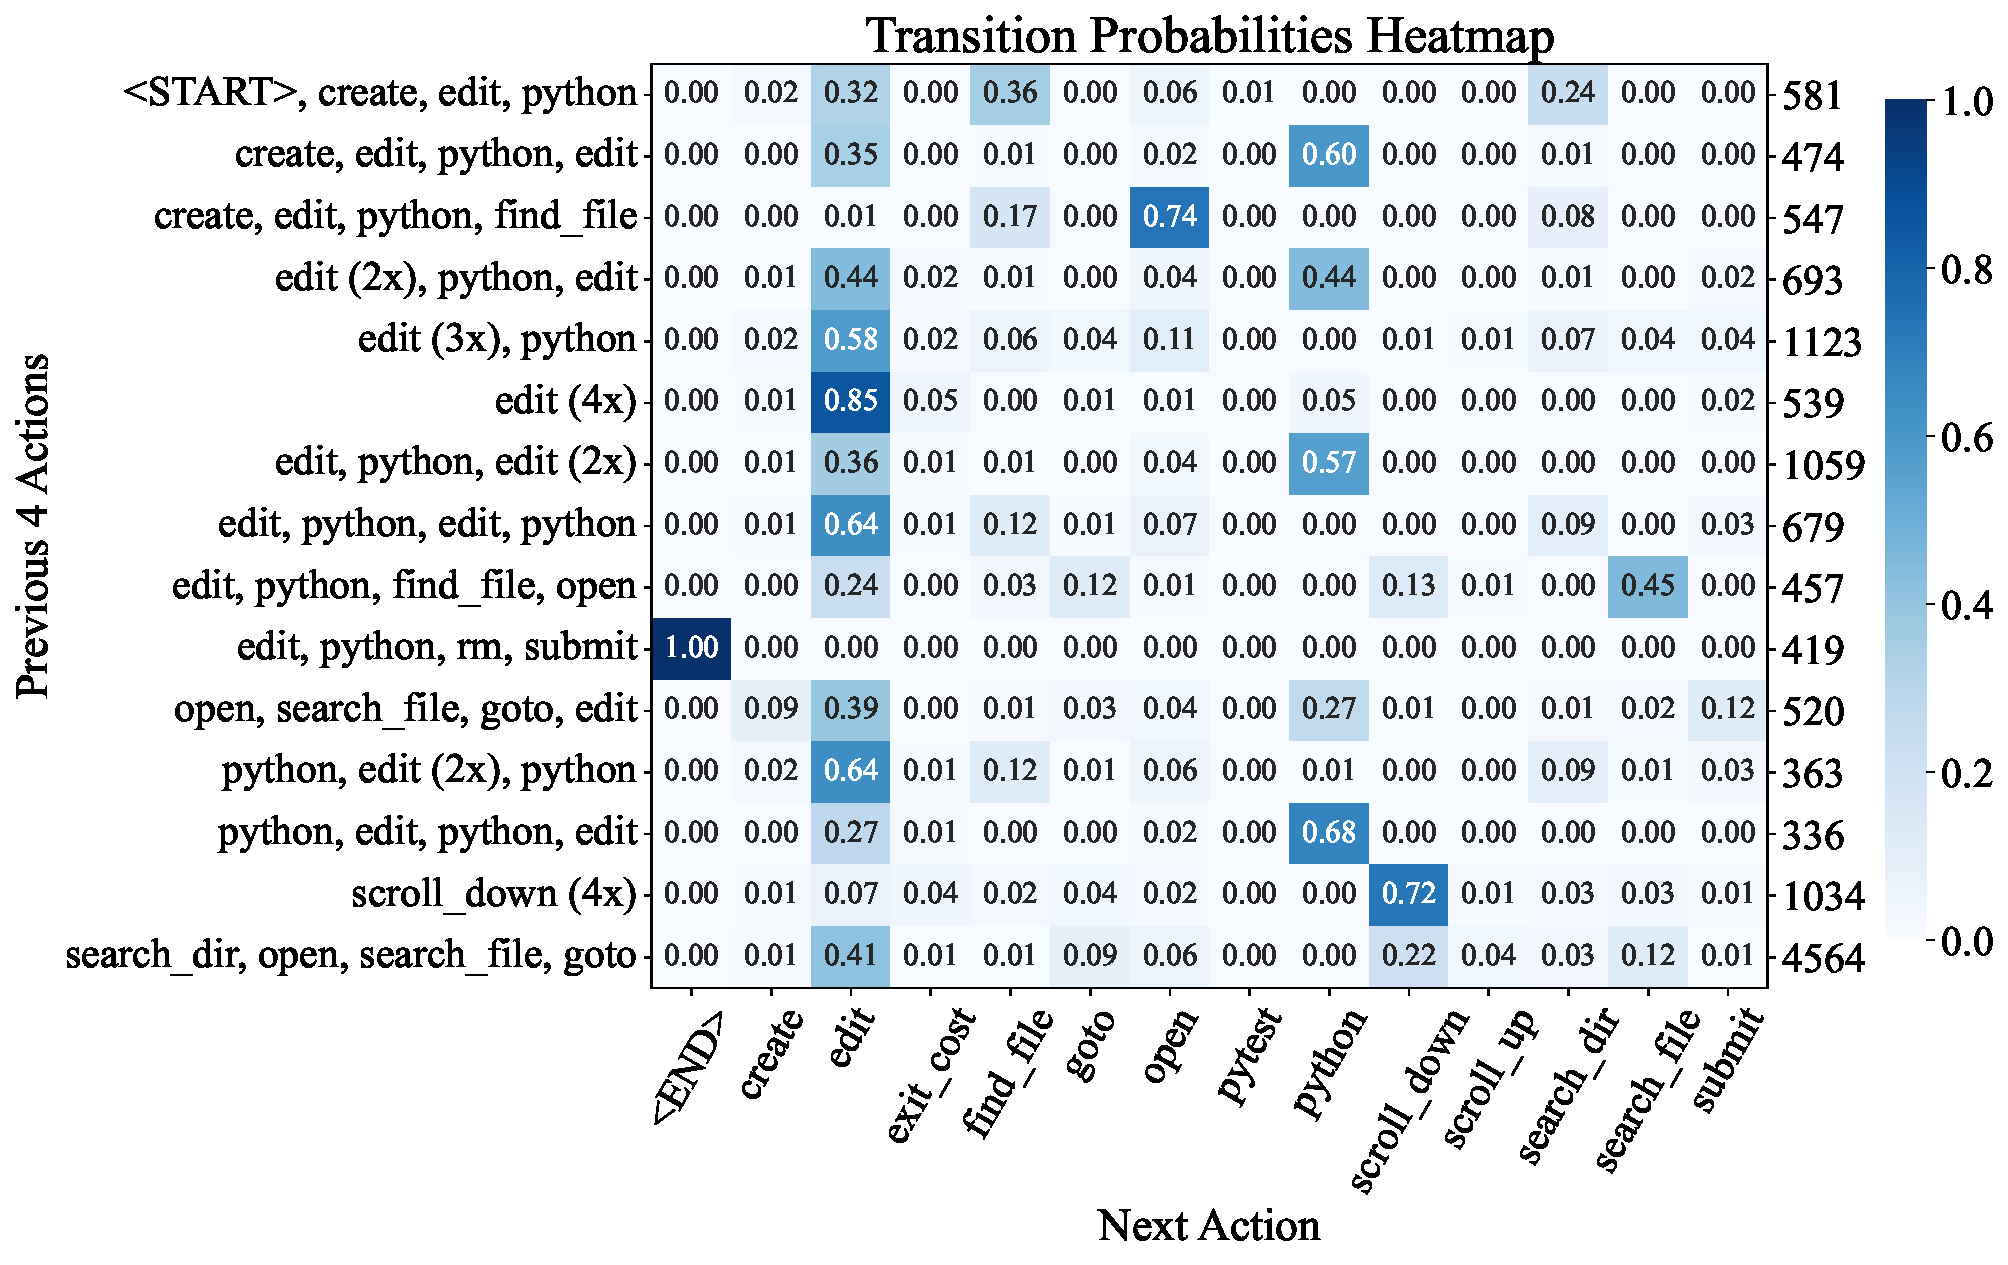
\includegraphics[width=\textwidth]{figures/appx/transition_probs_4gram.pdf}
    \caption{
    Heatmap displaying the relative frequency of different actions being invoked after the most popular \textit{quadruplets} of actions in SWE-agent w/ GPT-4 Turbo trajectories across all task instances.
    }
    \label{fig:transition_probs_4gram}
\end{figure}

Other interesting correlations are also present.
The edit/evaluate pattern is reflected in the correlation between the \texttt{edit} and \texttt{python} pair.
A variety of localization patterns are also conspicuous.
Sometimes, searching for a file turns out to be less fruitful than searching for a keyword, and visa versa.
This is reflected in the \texttt{find\_file} and \texttt{search\_dir} pair.
The invocation of \texttt{open} is representative of an agent honing in on a specific file to then continue localizing (\texttt{search\_file} \num{0.35}, \texttt{scroll\_down} \num{0.18}, \texttt{goto} \num{0.09}) or begin editing (\texttt{edit} \num{0.25}).

As the number of prior actions considered increases, more complex operations carried across multiple commands become apparent, echoing the observations from Table~\ref{tab:most_common_triples_by_index}.
In Figure~\ref{fig:transition_probs_3gram}, reproduction (e.g. [\texttt{create}, \texttt{edit}, \texttt{python}]) is typically followed by adjustments to the script (\texttt{edit} \num{0.39}) or localization (\texttt{find\_file} \num{0.31}, \texttt{search\_dir} \num{0.22}).
Fruitful localization patterns are once again reflected by [\texttt{find\_file} / \texttt{search\_dir}, \texttt{open}, \texttt{search\_file}] are followed by \texttt{goto}.
In Figure~\ref{fig:transition_probs_4gram}, the most popular \num{4}-grams are related to reproduction or editing.
The [\texttt{edit}, \texttt{python}, \texttt{rm}, \texttt{submit}] pattern is a popular way for trajectories to finish.
Common failure modes are also apparent; repeated actions like \texttt{edit} (\num{4}x) and \texttt{scroll\_down} (\num{4}x) typically continues cascading.